Standard LoRa (nazwa pochodzi od angielskich słów \textsl{Long Range}) należy do grupy systemów z~rozproszonym widmem
(ang. \textsl{Spread~Spectrum}) bazującą na technice \textsl{Chirp Spread Spectrum} (CSS). Wykorzystuje ona
szerokopasmowe impulsy typu \enquote{chirp} modulowane liniową częstotliwością w~celu kodowania przesyłanych informacji.
Sygnał jest sinusoidą, której częstotliwość wzrasta (\enquote{upchirp}) lub maleje (\enquote{downchirp}) w~czasie
\cite{semtech-lora-lorawan,ieee-802-15-4-2006}. LoRa jest technologią modulacji sygnałów przeznaczoną do budowania sieci
niskiej mocy o~dużym zasięgu (LPWAN, ang. \textsl{Low Power, Wide Area Network}).

Wykorzystanie LoRa pozwala na budowanie sieci, które mogą transmitować na bardzo duże odległości -- teoretycznie do 5~km
w~terenach zabudowanych oraz do 15 km na terenach otwartych \cite{semtech-lora-lorawan}, zużywając przy tym małe ilości
energii. Zaprojektowana z~myślą o~urządzeniach wykorzystujących zasilanie bateryjne w~celu podłączenia ich bezprzewodowo
do lokalnych, regionalnych lub globalnych sieci. Standard wykorzystuje transmisje na bezlicencyjnych częstotliwościach
radiowych poniżej 1~GHz -- przykładowo w~Europie jest to 868 MHz (EU868), natomiast w~Ameryce Północnej 915 MHz (US915).

Zgodnie z~definicją siedmiowarstwowego Modelu Referencyjnego OSI dla sieci, którego schemat przedstawia rys.
\ref{img:osi-seven-layer}, standard LoRa jest wyłącznie implementacją warstwy fizycznej (PHY, ang. \textsl{physical
    layer}). W~modelu tym wyróżnia się następujące warstwy (w kolejności od najwyższej) \cite{osi-model}:
\begin{itemize}[label=--]
    \item warstwa 7, aplikacyjna: odpowiada za interakcję człowiek-komputer, warstwa, gdzie aplikacja ma dostęp do sieci,
    \item warstwa 6, prezentacyjna: zadbanie o~użyteczny format danych, szyfrowanie danych,
    \item warstwa 5, sesyjna: utrzymanie połączeń, kontrola nad portami oraz sesjami,
    \item warstwa 4, transportowa: transmisja danych wykorzystując do tego odpowiednie protokoły,
    \item warstwa 3, sieciowa: zarządzanie trasami przesyłania danych,
    \item warstwa 2, łącza danych (kanałowa): definiowanie formatu przesyłanych danych,
    \item warstwa 1, fizyczna: przesyłanie logicznych zer oraz jedynek (pojedynczych bitów).
\end{itemize}

\begin{figure}[!htbp]
    \centering
    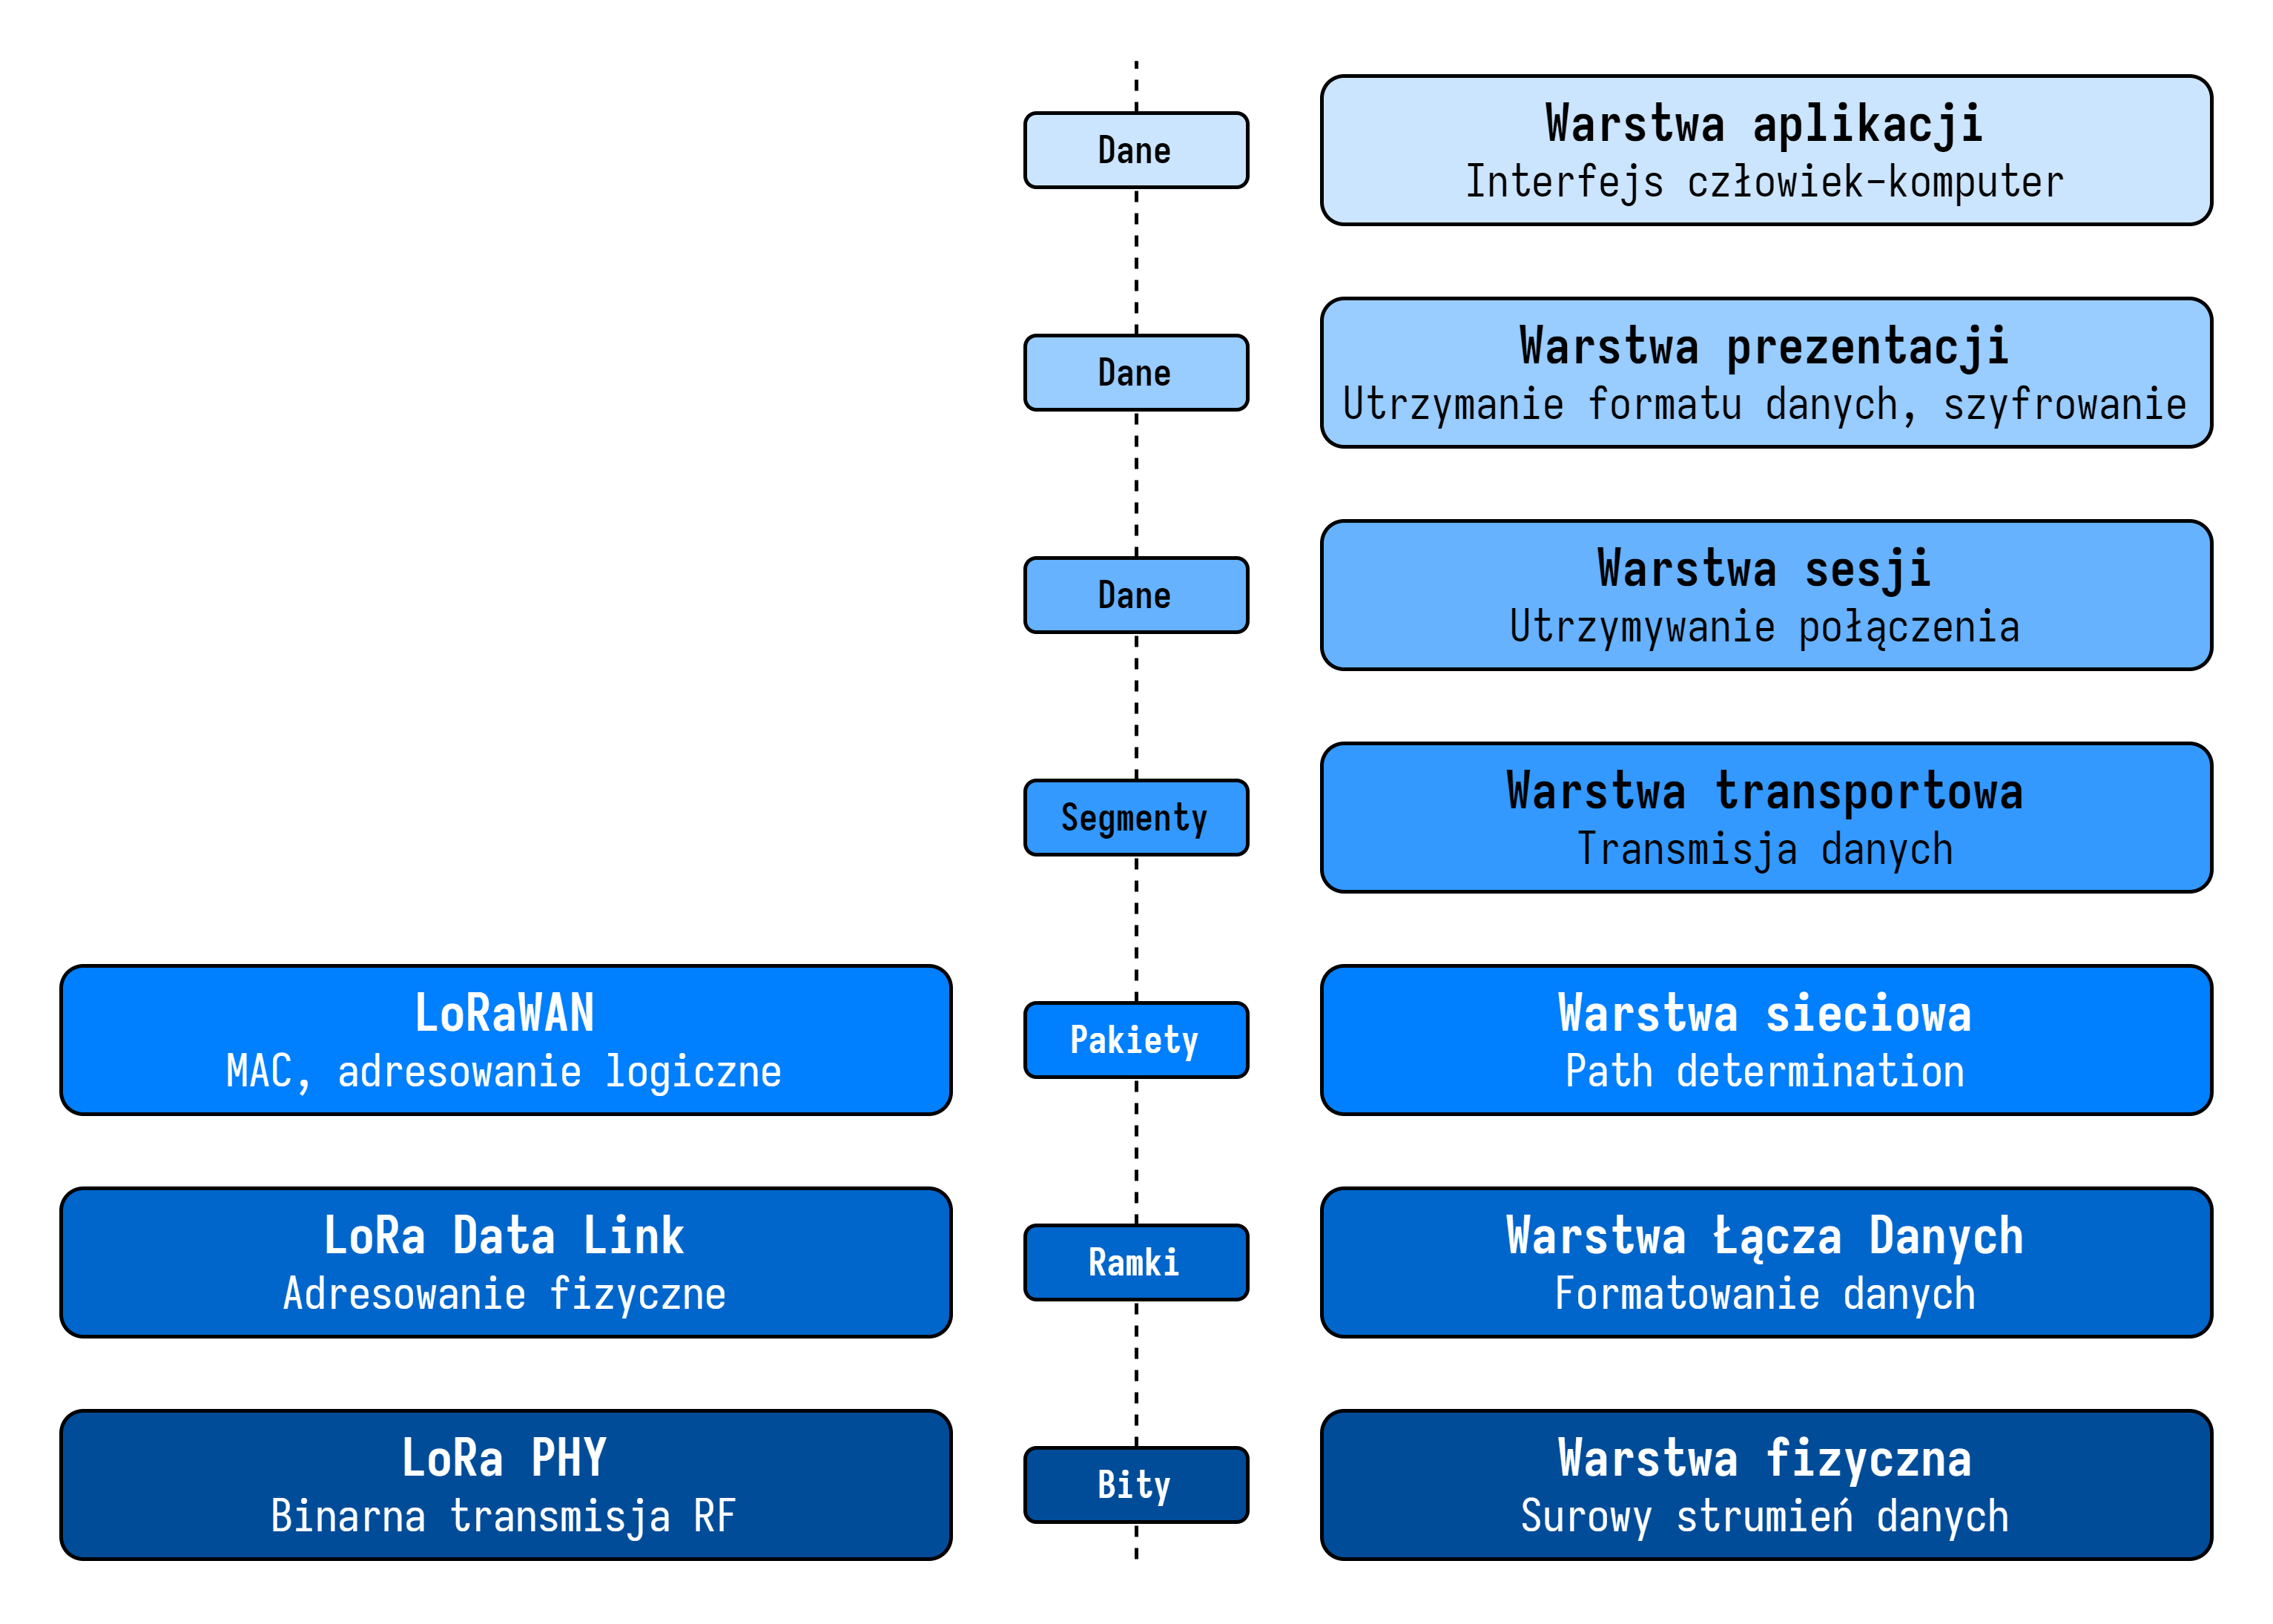
\includegraphics[width=0.8\textwidth]{schematics/osi-seven-layers}
    \caption{\label{img:osi-seven-layer}Schemat siedmiowarstwowego modelu OSI}
\end{figure}

\FloatBarrier
Wykorzystując standard LoRa, możliwe jest zbudowanie prostych sieci, w~których komunikacja odbywa się bezpośrednio
pomiędzy modułami sieci metodą urządzenie-urządzenie (D2D, ang. \textsl{device-to-device}). Sieć taka będzie miała
ograniczone możliwości weryfikacji integralności (spójności) danych. Sama warstwa fizyczna nie posiada żadnego
mechanizmu rozpoznawania wysyłanych lub odbieranych danych, dostępne są tylko kody CRC (ang. \textsl{Cyclic Redundancy
    Check}), które pozwalają tylko na zero-jedynkowe określenie czy wystąpił błąd, bez możliwości określenia, w~którym
momencie wystąpił czy podjęcia próby naprawienia go. Topologiami, które można zastosować, są topologia gwiazdowa (ang.
\textsl{star}) -- jeden moduł centralny, z~którym bezpośrednio komunikują się pozostałe urządzenia lub topologia siatki
(ang. \textsl{mesh}) -- moduły połączone są ze sobą w~grupy (np. na podstawie ich lokalizacji), transmisje odbywają się
na zasadzie ogłoszeń i~przesyłane dalej do momentu, gdy dotrą do adresata. Schematy takich topologii przestawione
zostały na rys. \ref{img:network-topologies}.

\begin{figure}[!htbp]
    \centering
    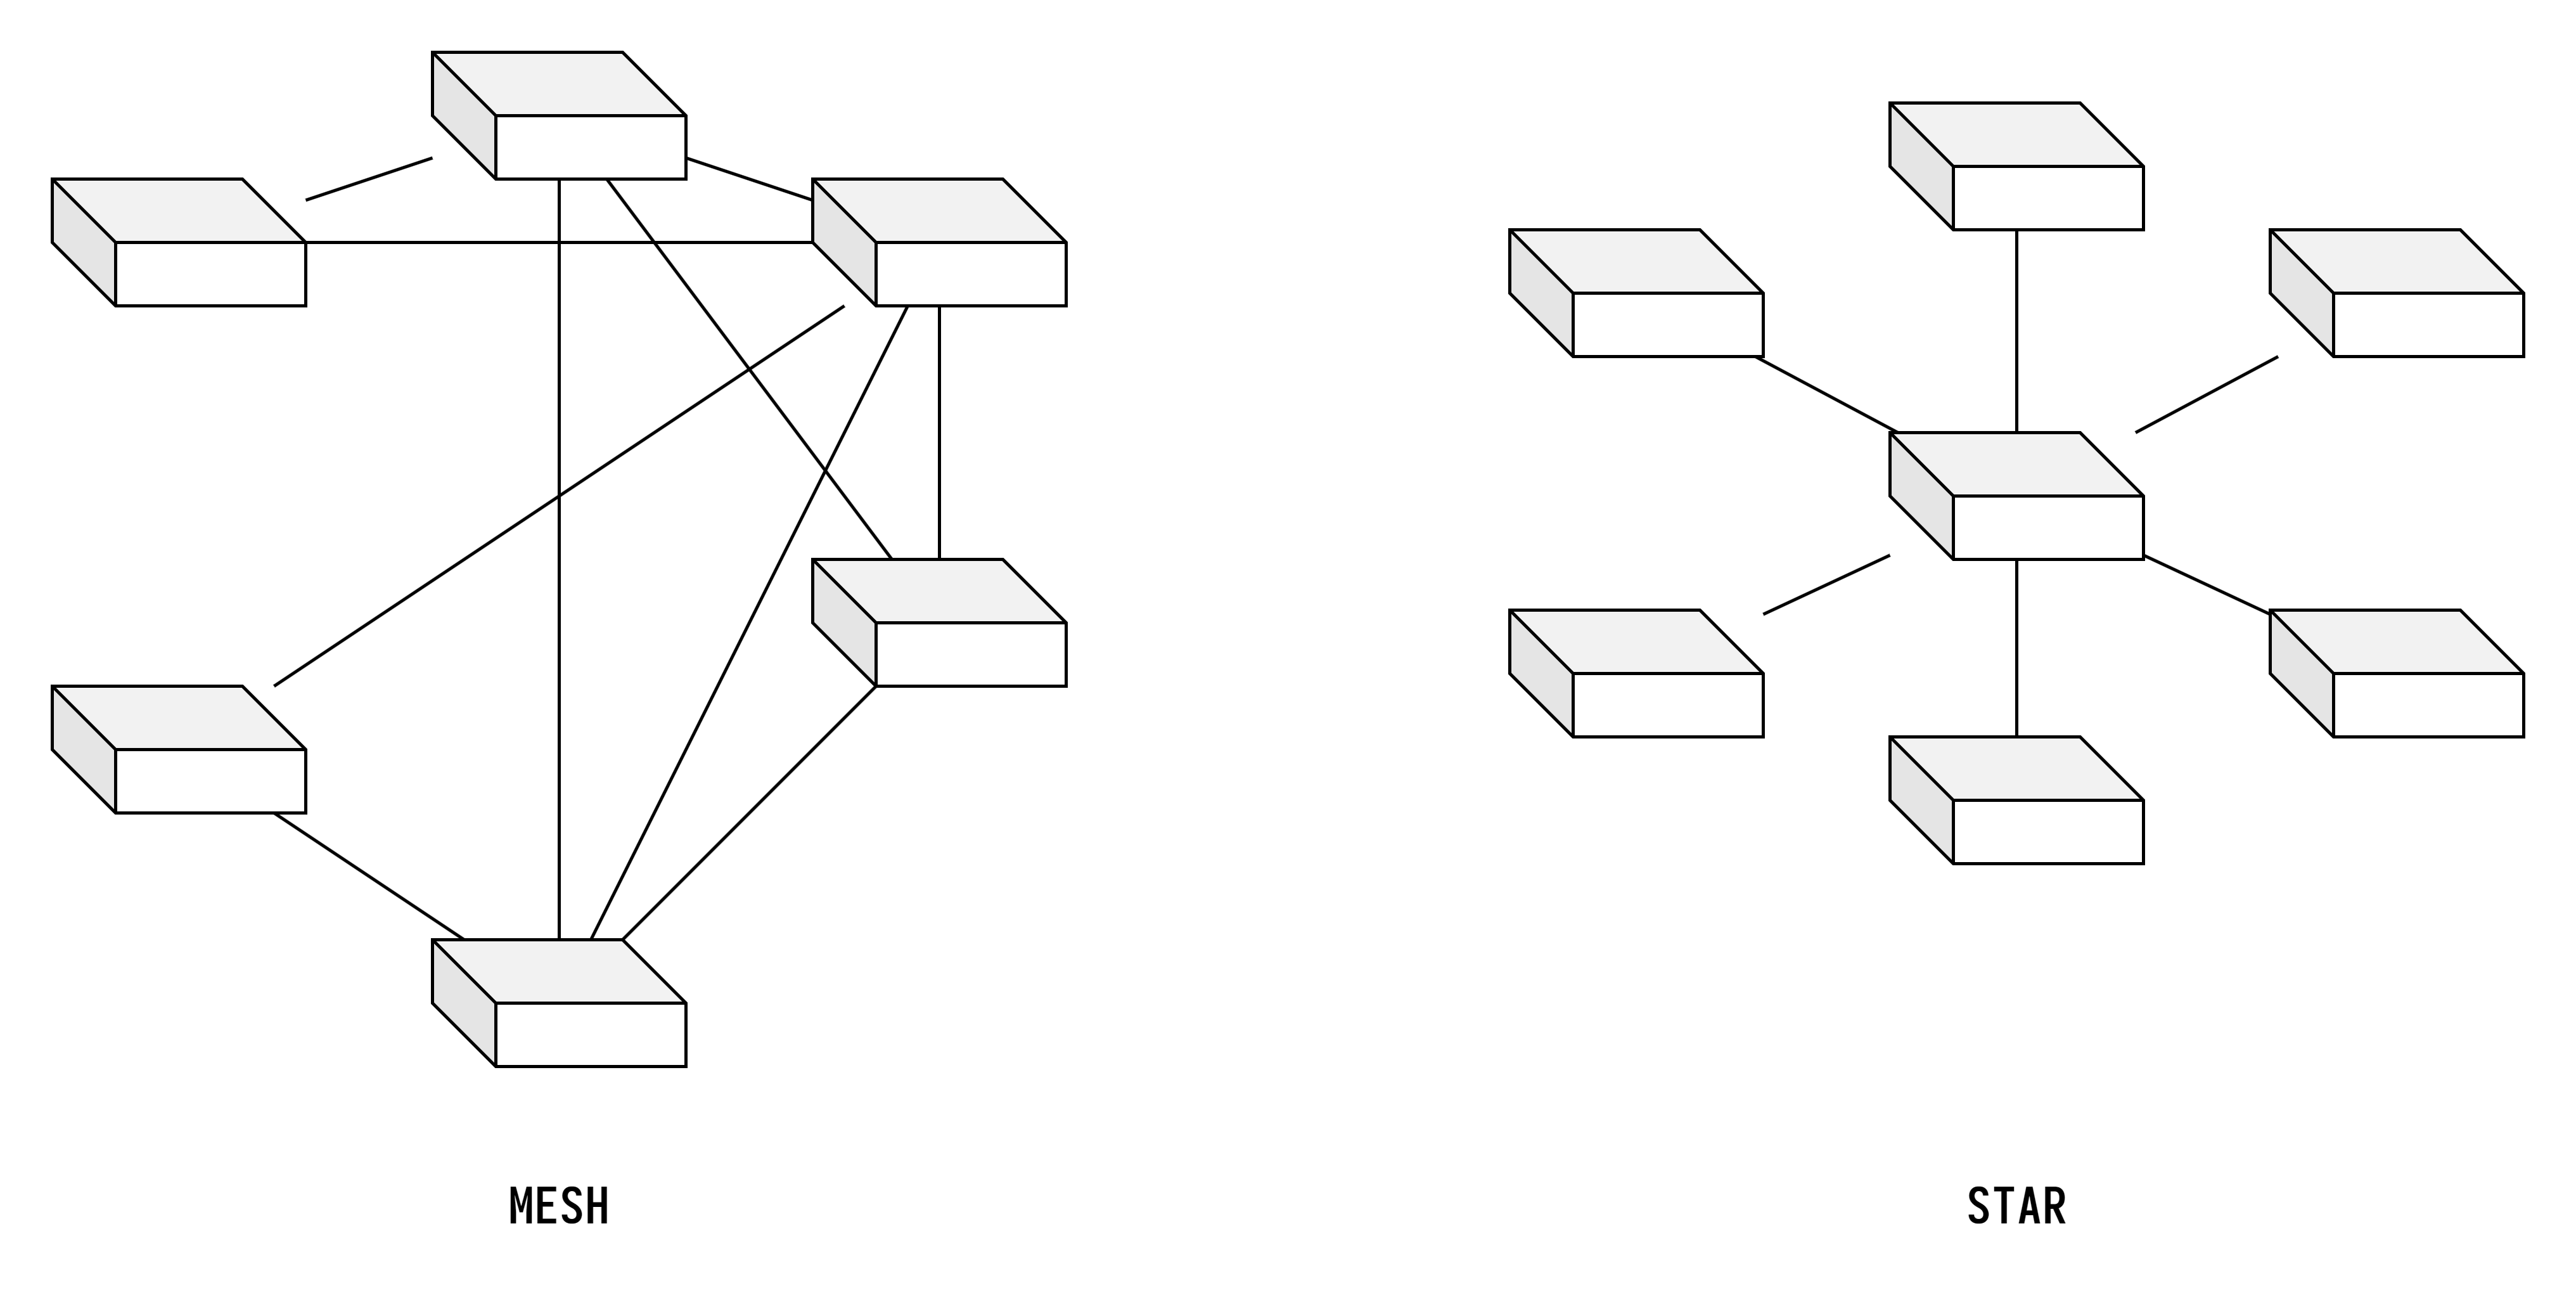
\includegraphics[width=0.8\textwidth]{schematics/network-topologies}
    \caption{\label{img:network-topologies}Schematy sieci w~topologiach mesh oraz gwiazdowej}
\end{figure}

\FloatBarrier
\section{\label{sect:lora-modulation}Modulacja LoRa Spread Spectrum} W~modulacji LoRa rozproszenie widma uzyskiwane jest
dzięki generowaniu sygnałów typu chirp (tzw. \enquote{świergotach}), które posiadają ciągłą zmianę w~ich częstotliwości.
Przy wykorzystaniu takiej metody przesunięcia w~czasie oraz częstotliwości są identyczne dla nadajnika, jak
i~odbiornika, dzięki czemu złożoność konstrukcji odbiornika może być znacznie zredukowana \cite{lora-modulation-basics}.
Ponadto LoRa wykorzystuje rozproszenie ortogonalne (prostopadłe), co pozwala urządzeniom pracującym w~sieci na dodatkowe
oszczędzanie energii poprzez dostosowanie swoich parametrów pracy w~stosunku do potrzeb.

Jedna ramka transmisji LoRa składa się z~ciągu zmodulowanych symboli $s(nT_s)$, zgodnie z~zależnością
\cite{lora-modulation-fscm,lora-emulator}:
\begin{equation}
    x(t) = \sum_{n=1}^{N_M} s_n(t-nTs)\text{,}
\end{equation}
gdzie $N_m$ jest całkowitą ilością symboli w~przesyłanej ramce.

Modulacja bazuje na cyklicznych (powtarzających się) sygnałach, a~przesunięcia w~stosunku do częstotliwości nośnej
(\enquote{pozycji startowej}) pozwalają na zakodowanie wartości symbolu. Parametrem pozwalającym na kontrolę
częstotliwości chirpów jest \textsl{speading factor} ($\mathrm{SF}$). W~przypadku regionu europejskiego wartość ta może
zostać wybrana z~przedziału \{7,8,9,10,11,12\}. Im większa jego wartość, tym dłużej trwa przesłanie jednego sygnału, co
w~efekcie pozwala na przesłanie większej ilości bitów w~jednym symbolu. Jeden chirp (\enquote{świergot}) w~standardzie
LoRa zaprojektowany został do odzwierciedlenia $M=2^{\mathrm{SF}}$ wartości symboli, gdzie ich czas trwania (długość)
dana jest w~postaci $T_s=M/\mathrm{BW}$, a~wartość $\mathrm{BW}$ przedstawia wykorzystaną szerokość pasma
\cite{lora-modulation-fscm}. LoRa wykorzystuje zadane wartości szerokości pasma, z~przedziału
$\mathrm{BW}$=\{125,250,500\} kHz, przy czym ich dostępność zależna jest od tego, gdzie sieć operuje i~jest regulowana
\cite{lora-regional-parameters}, tak samo, jak inne parametry sieci, przez LoRa Alliance. Zmodulowany przez LoRa
przebieg można przedstawić analitycznie \cite{lora-emulator} w~postaci równania:
\begin{equation}\label{eqn:lora-waveform}
    s(t) = \exp{\left({j}2\pi\int_{0}^{t}\left[(\beta x+\gamma_n)_{\bmod{_{\mathrm{BW}}}}-\frac{\mathrm{BW}}{2}\right]\,dx\right)}\text{,}
\end{equation}
gdzie $\gamma_n$ to przesunięcie częstotliwości, które można wyznaczyć, korzystając z~zależności:
\begin{equation}
    \gamma_n = m_n\Delta_f = \frac{m_n}{T_s}\text{,}
\end{equation}
gdzie $m_n$ jest wartością symbolu z~przedziału $m_n\in\{0,1,\ldots,M-1\}$, $n$ jest indeksem symbolu, a $\Delta_f$
przedstawia krok między zmianami częstotliwości.

W~przypadku LoRa krok w~zmianie częstotliwości wybrany został jako częstotliwość pojedynczego symbolu $B/M$. Kolejnym
ważnym dla modulacji LoRa parametrem jest tzw. \enquote{częstotliwość świergotania} (ang. \textsl{Chirp Rate}).
Odpowiednio dobrany, pozwala na separację symboli oraz uniknięcie zakłóceń międzysymbolowych (ISI, ang.
\textsl{Inter-Symbol Interference}). Wyznaczany jest na podstawie czasu trwania jednego symbolu $T_s$ w~danym paśmie
transmisyjnym $\mathrm{BW}$, tak aby każdy symbol zaczynał się oraz kończył na takiej samej częstotliwości:
\begin{equation}
    \beta = \frac{f_{\mathrm{high}}-f_{\mathrm{low}}}{T_s}=\frac{\mathrm{BW}}{T_s}\text{,}
\end{equation}
gdzie $f_{\mathrm{high}}\ \text{oraz}\ f_{\mathrm{low}}$ to odpowiednio górna i~dolna granica częstotliwości
pojedynczego świergotu. W~przypadku, gdy wartość $\beta > 0$, sygnał będzie typu upchirp (o częstotliwości rosnącej),
natomiast typu downchirp (o częstotliwości malejącej) dla $\beta < 0$. Reprezentacja dwóch symboli LoRa
\cite{lora-emulator} przedstawiona zotała na rys. \ref{img:upchirp-lora-modulated-symbol}. Dzięki zastosowaniu takiej
modulacji, energia sygnału rozproszona jest w~większym paśmie transmisyjnym, co pozwala na znaczne zredukowanie
wąskopasmowych zakłóceń (ang. \textsl{narrow-band interferences}). W~przypadku, gdy do transmisji wybrana zostanie
wyższa wartość SF, zwiększa się czułość odbiornika z~uwagi na zwiększoną energię symbolu, jednakże skutkuje to
zmniejszeniem przepustowości sieci oraz zwiększonym zużyciem energii przez moduły \cite{css-modulation-technique}.

\begin{figure}[!htbp]
    \centering
    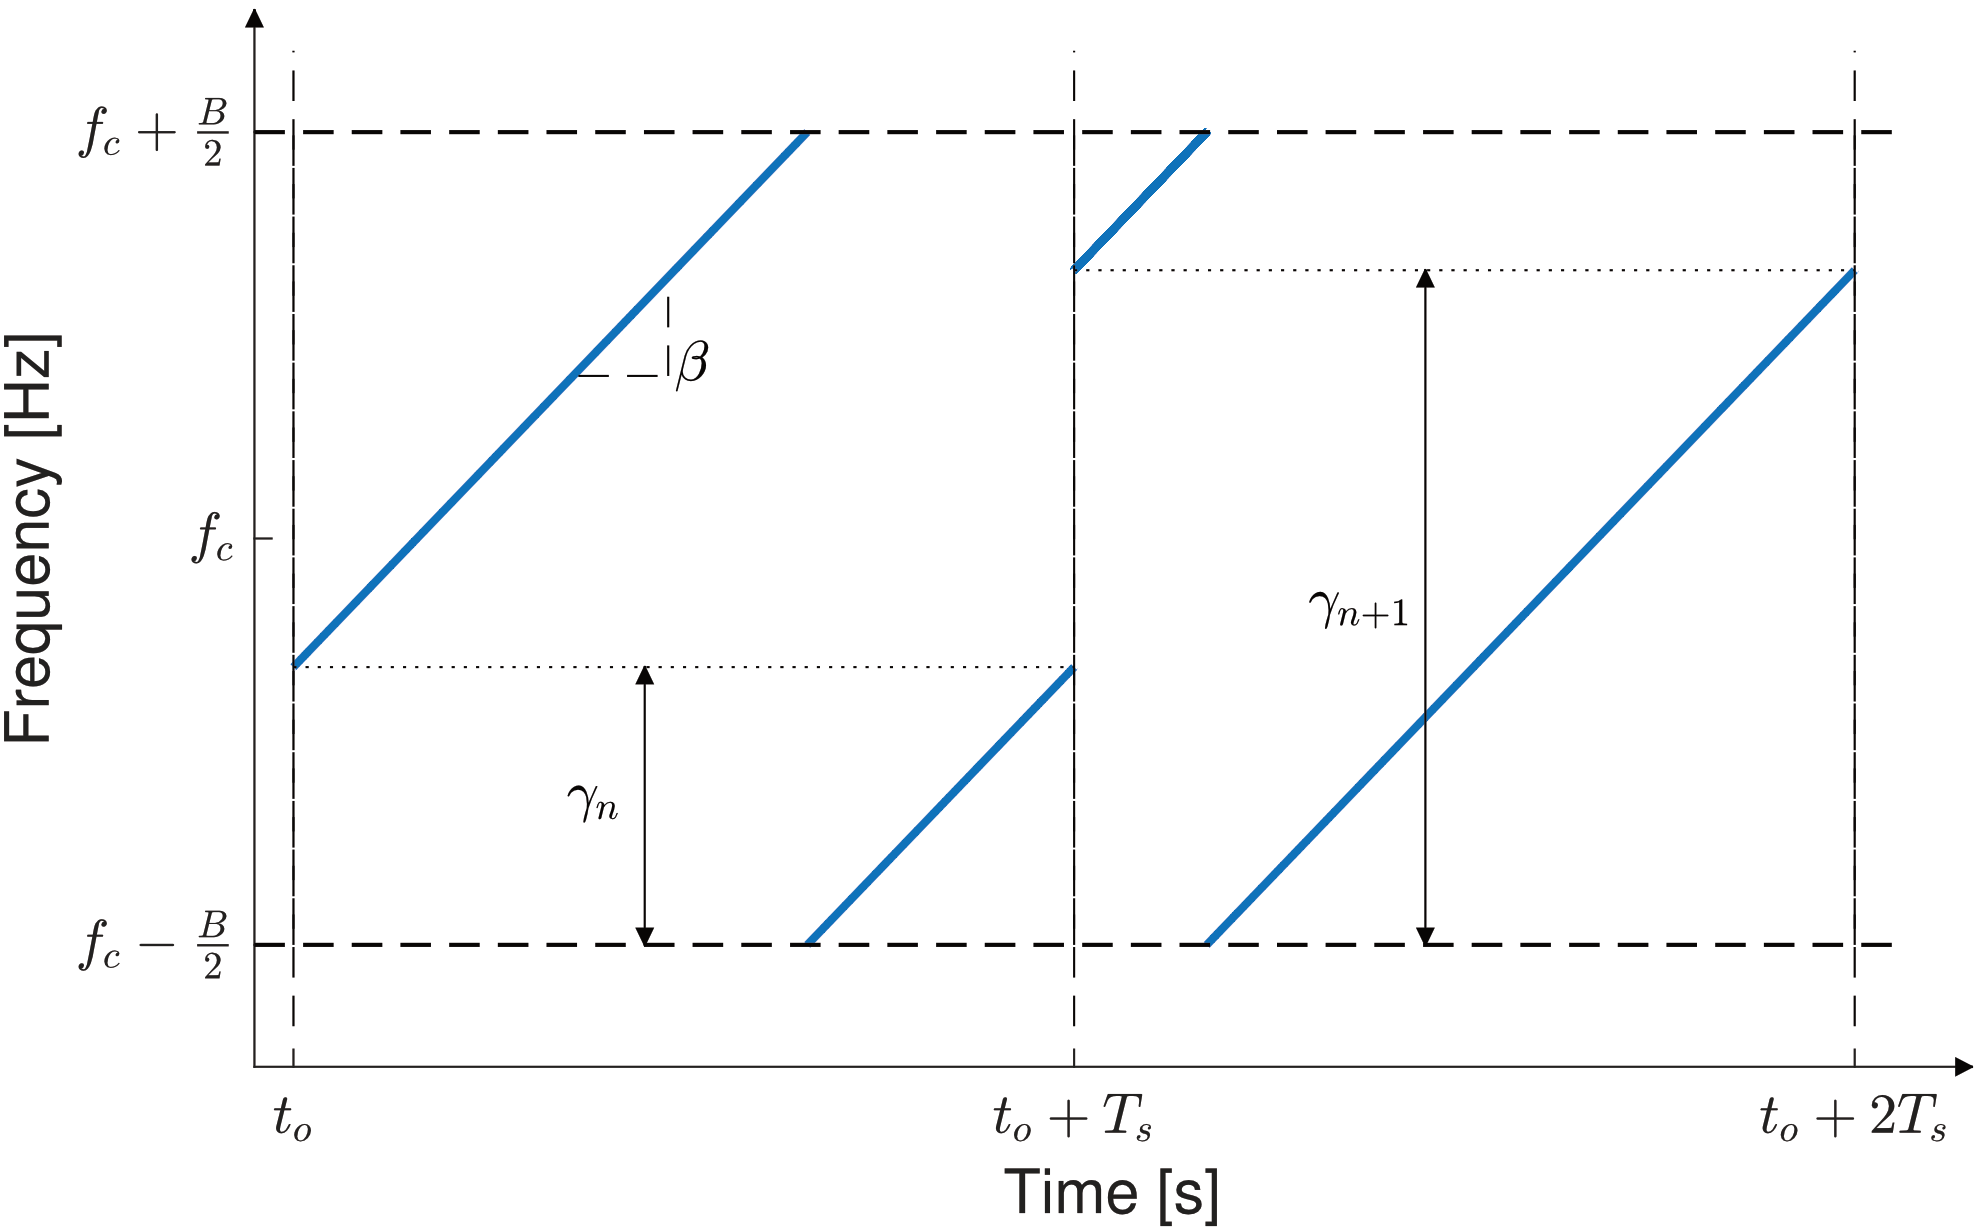
\includegraphics[width=0.9\textwidth]{theory/upchirp-lora-modulated-symbol}
    \caption{\label{img:upchirp-lora-modulated-symbol}Przebieg dwóch symboli typu upchirp w~modulacji LoRa, ilustracja
        wykorzystana zgodnie z~licencją publikacji \cite{lora-emulator}}
\end{figure}

\FloatBarrier

\section{\label{sect:lorawan}Wyższe warstwy -- protokół LoRaWAN} LoRaWAN to ustandaryzowany, otwarty protokół sieciowy,
za którego utrzymanie odpowiada LoRa Alliance (do którego należą m.in. Semtech oraz ST Microelectronics). Obecnie
aktualną wersją jest 1.0.4 (październik 2020). Protokół definiuje górne warstwy sieci wykorzystujących warstwę fizyczną
LoRaPHY. Wykorzystując go, możliwe jest budowanie sieci zapewniających komunikację dwukierunkową pomiędzy modułami
(urządzeniami końcowymi), bramami oraz serwerami. Na LoRaWAN składa się kilka elementów tworzących jej stos
technologiczny (ang. \textsl{technology stack}). Jego schemat przedstawiony został na rys. \ref{img:lorawan-technology}.

\begin{figure}[!htbp]
    \centering
    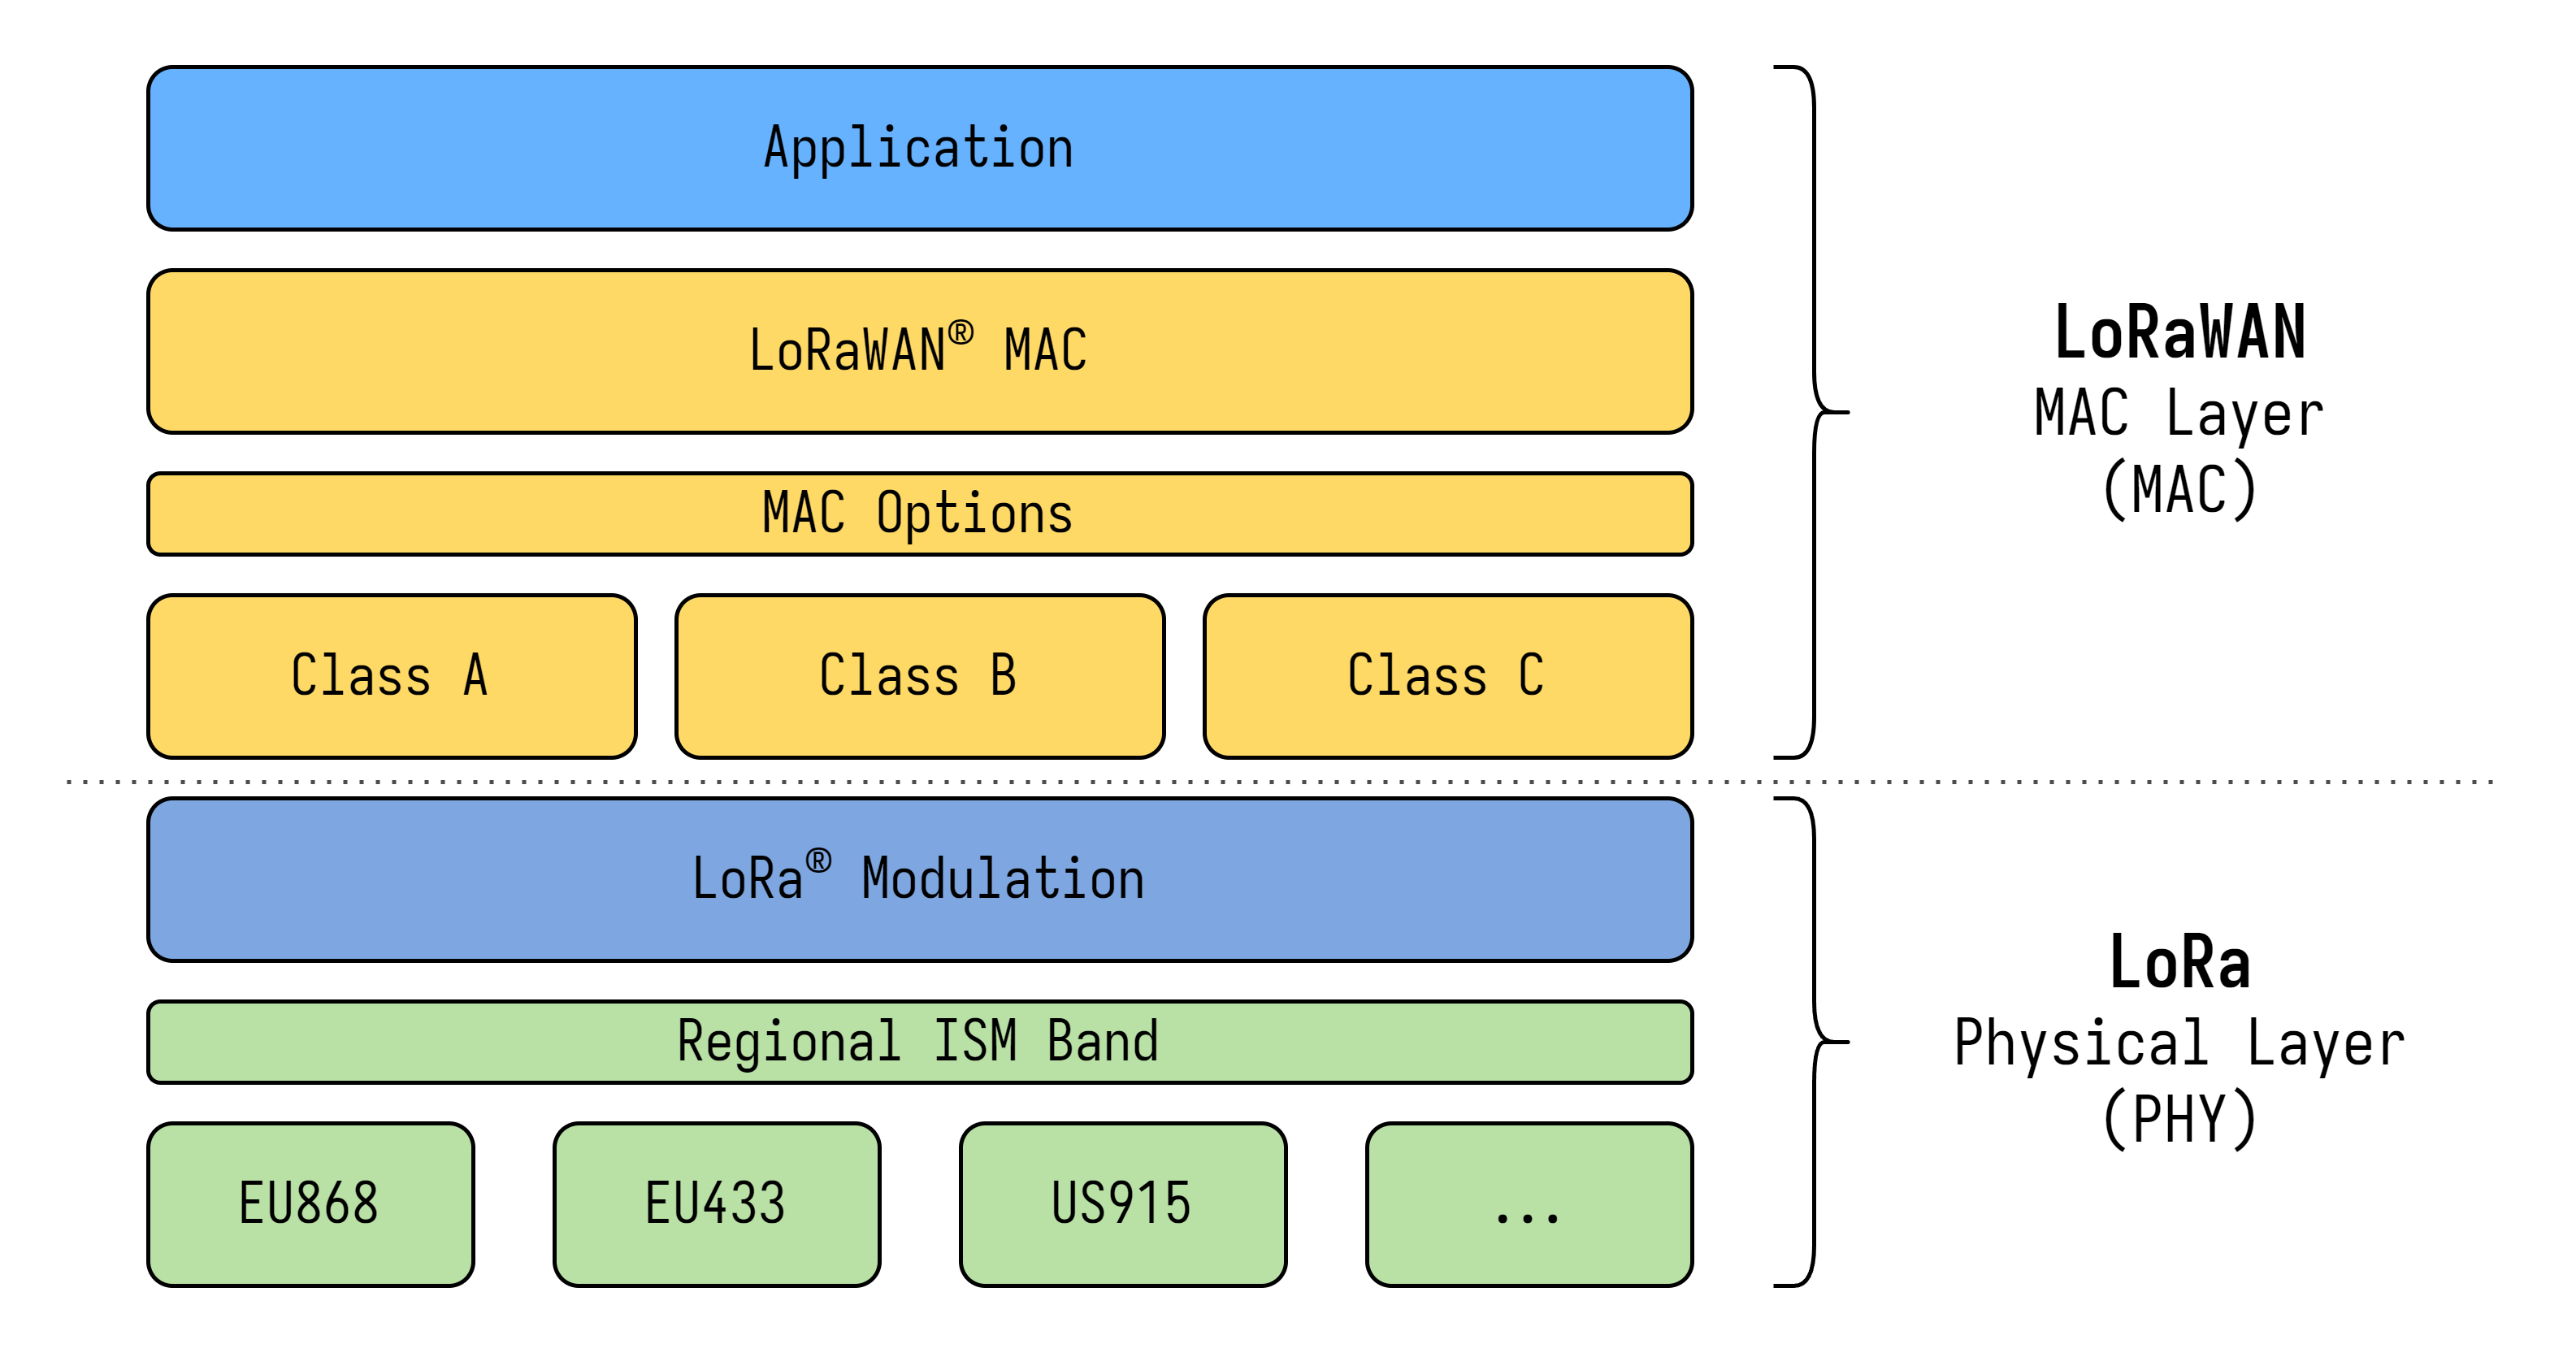
\includegraphics[width=0.8\textwidth]{schematics/lorawan-technology}
    \caption{\label{img:lorawan-technology}Schemat stosu technologicznego sieci wykorzystujących LoRaWAN}
\end{figure}

Widoczne na schemacie klasy (A, B, C) określają tryb pracy urządzeń operujących w~sieci LoRaWAN. Wszystkie urządzenia
muszą spełniać operację w~klasie A, urządzenia klasy B~muszą móc operować w~klasie B~oraz klasie A, natomiast
w~przypadku urządzeń klasy C -- muszą one operować w~każdej z~klas \cite{lorawan-device-class,lorawan-classb-eval}.

Podstawowa klasa -- klasa A~przewiduje 3~okna transmisyjne, 1~na transmisję do sieci (uplink) oraz 2~na odbieranie
danych (downlink). Urządzenia klasy A~nie mogą być aktuatorami, ponieważ to one rozpoczynają wymianę danych w~sieci.
Podczas normalnej pracy urządznie jest w~stanie spoczynku. W~momencie, gdy wystąpi zmiana w~jego otoczeniu, wysyłane są
dane do sieci w~oknie Tx. Następnie urządzenie oczekuje na odpowiedź. Jeżeli nie dostanie jej w~oknie Rx1 (pierwszym
oknie odbierania), to na krótki czas przechodzi w~stan spoczynku, po czym wybudza się, oczekując na odpowiedź w~oknie
Rx2 (drugim oknie odbierania). W~przypadku klasy A, urządzenie nie będzie próbowało ponownie nadawać, jeżeli dostanie
odpowiedź w~pierwszym oknie (Rx1) lub jeżeli drugie okno po ostatniej transmisji (Rx2) zostanie zakończone.

Klasa B~urządzeń oferuje możliwość pracy na zaplanowanym harmonogramie z~określonymi, stałymi w~czasie, oknami na
odbieranie danych \cite{lorawan-classb-eval}. W~przeciwieństwie do klasy A, urządzenia klasy B~nadają się do pracy jako
sensory oraz jako aktuatory. Praca w~klasie B~jest oparta na procesie nazywanym \textsl{beaconing}. Zsynchronizowane
czasowo urządzenie (\textsl{beacon}) okresowo nadaje w~sieci poprzez bramy i~dzięki temu urządzenia końcowe
synchronizują swój wewnętrzny zegar. Dzięki synchronizacji urządzenia mogą nasłuchiwać tylko w~określonych momentach,
mając pewność, że w~momencie otwarcia swojego okna mogą się spodziewać odbioru danych.

Urządzenia klasy C~operując w~trybie \enquote{zawsze włączone}, więc najczęściej nie są oparte o~zasilanie bateryjne.
W~tym przypadku są one w~stanie ciągłego nasłuchu, pod warunkiem, że same nie nadają wiadomości do sieci. W~klasie
C~zaimplementowane zostały takie same okna jak w~przypadku klasy A, z~tą różnicą, że okno Rx2 nie zostaje przerwane aż
do momentu, gdy urządzenie końcowe zaczyna samo nadawać i~trwa jego okno Tx. Dzięki temu urządzenia mogą otrzymywać
wiadomości w~prawie każdej chwili.

\FloatBarrier
\subsection{\label{sect:lorawan-architecture}Architektura sieci LoRaWAN} Na sieci oparte o~protokół LoRaWAN składa się
więcej elementów niż w~przypadku sieci wykorzystujących tylko warstwę fizyczną. Należą do nich: urządzenia końcowe,
bramy oraz kilka rodzajów serwerów. Implementacja takie rozwiązania jest przez to bardziej złożona, ale zapewnia dzięki
temu większe możliwości przykładowo mniejszy wpływ terenu na komunikację lub szyfrowanie przesyłanych danych.
Przykładowy schemat architektury sieci LoRaWAN przedstawiony został na rys. \ref{img:lorawan-architecture}.

\begin{figure}[!htbp]
    \centering
    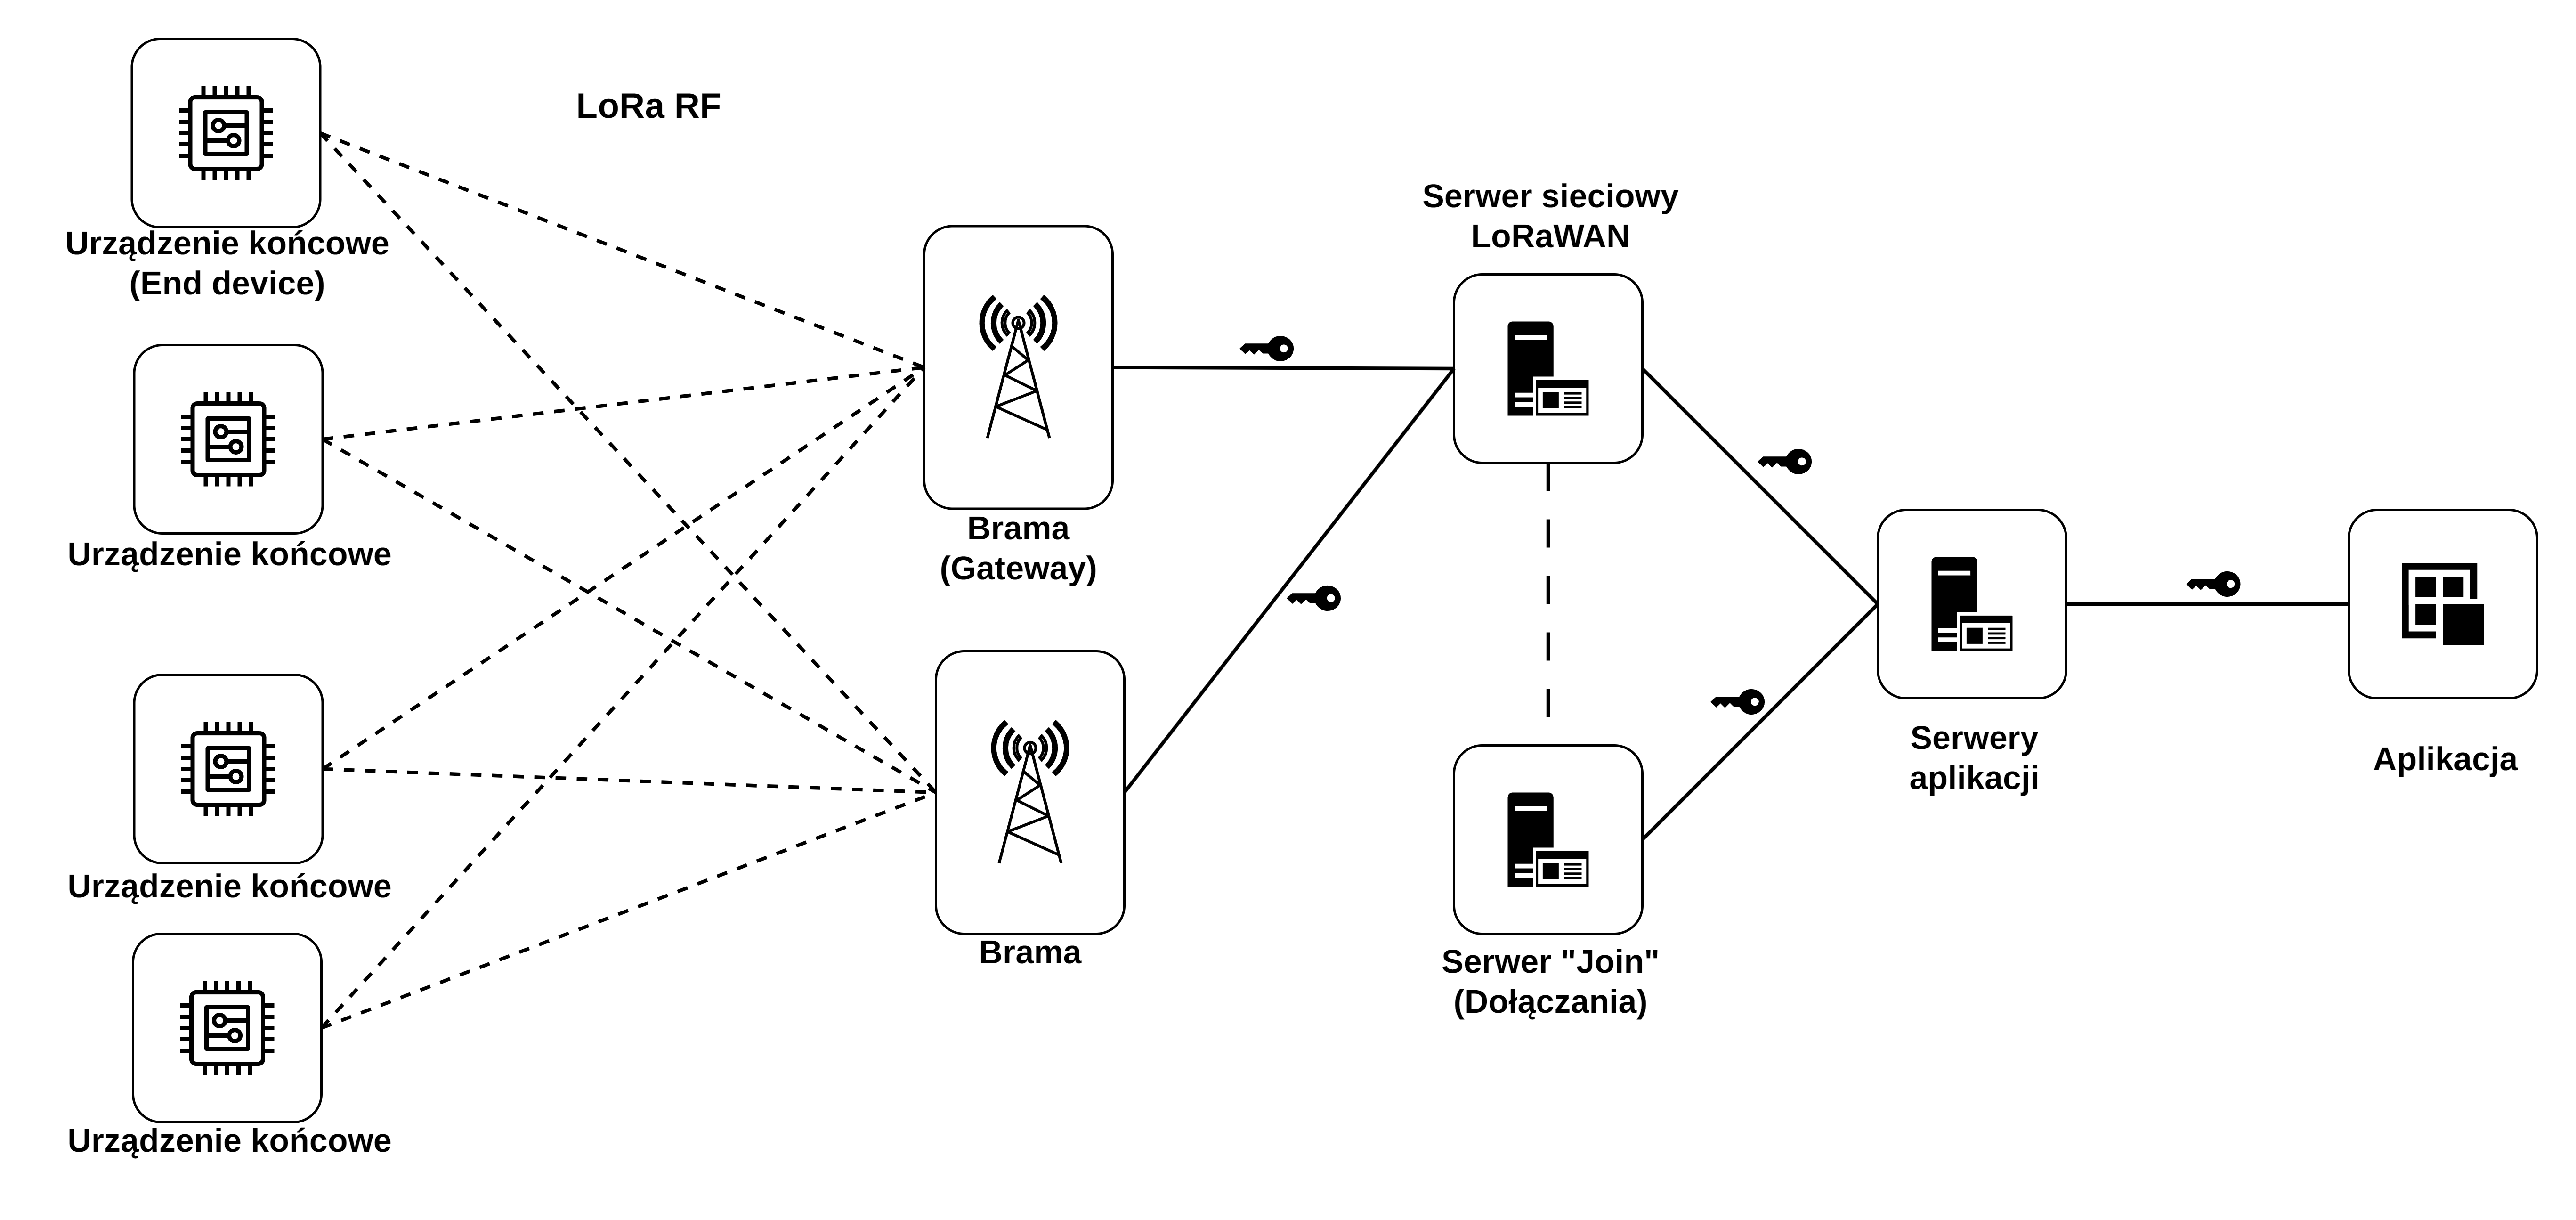
\includegraphics[width=\textwidth]{schematics/lorawan-architecture}
    \caption{\label{img:lorawan-architecture}Schemat architektury sieci LoRaWAN}
\end{figure}

Urządzeniem końcowym może być np. sensor, który zbiera dane ze swojego otoczenia. Takie urządzenie pracuje najczęściej
na zasilaniu bateryjnym. Jeżeli jest ono urządzeniem wyposażonym w~możliwość komunikacji przez LoRa, to podczas jego
produkcji przypisywany jest mu unikalny identyfikator. Pozwala on przykładowo na zarządzenie urządzeniem w~sieci oraz
bezpieczną transmisję danych do sieci.

Bramą (ang. \textsl{Gateway}) jest urządzenie, które odbiera zmodulowany sygnał LoRa od dowolnego urządzenia w~jego
zasięgu i~przekazuje go do dalszych elementów sieci -- serwerów sieciowych LoRaWAN. Nie występuje tutaj bezpośrednie
przypisanie urządzeń do konkretnych bram, a~każde urządzenie końcowe może być obsługiwane przez wiele bram w~danym
obrębie sieci. Dzięki temu poziom błędu pakietów jest znacznie niższy, ponieważ jest bardzo duża szansa, że przynajmniej
jedna brama poprawnie odbierze wiadomość nadawaną przez urządzenie końcowe.

Pierwszym typem serwera jest serwer sieciowy LoRaWAN (LNS, ang. \textsl{LoRaWAN network server}). Urządzenie to zarządza
całą siecią. Dynamicznie modyfikuje parametry w~zależności od zmieniających się warunków oraz zapewnia bezpieczne,
szyfrowane 128-bitowym standardem AES (ang. \textsl{Advanced Encryption Standard}) połączenie między elementami sieci
(urządzeniami końcowy a~serwerem aplikacji). Drugim typem serwera są serwery aplikacyjne (ang. \textsl{Application
    server}), których zadaniem jest bezpiecznie odbieranie, zarządzanie oraz interpretacja danych z~sieci. Ponadto
odpowiedzialne są za generowanie pakietów, które potem przesyłane są do urządzeń końcowych. Ostatnim typem serwera są
serwery \textsl{Join} -- ich zadaniem jest zarządzanie procesem uruchamiania połączenia do sieci dla urządzeń końcowych,
które wyślą prośbę o~dołączenie.